\documentclass[12pt]{article}

%% Language and font encodings
\usepackage[english]{babel}
\usepackage[utf8x]{inputenc}
\usepackage[T1]{fontenc}
\usepackage{fancyhdr}

%% Sets page size and margins
\usepackage[a4paper,top=3cm,bottom=2cm,left=3cm,right=3cm,marginparwidth=1.75cm]{geometry}

%% Packages
\usepackage{xcolor}
\usepackage[colorlinks=true, allcolors=red]{hyperref}
\usepackage{lipsum}
\usepackage{graphicx}
\usepackage{float}
\usepackage[all]{hypcap}
\usepackage{changepage}
\usepackage{amsmath}
\usepackage{amsthm}
\usepackage{amssymb}
\usepackage{xspace}
\usepackage{tikz}

%% Other
\graphicspath{{Figures/}}
\setlength\parindent{0pt}
\newcommand{\auth}{Giulia Baldini, Luis Fernandes, Agustin Vargas Toro}
\newcommand{\ass}{Assignment 3}

%% Page settings
\pagestyle{fancy}
\fancyhf{}
\rhead{\auth}
\lhead{\ass}
\rfoot{\thepage}

\title{Foundations of Audio Signal Processing\\ \ass}
\author{\auth}

\begin{document}
	\maketitle
	\section*{Exercise 3.1}
	\textbf{a.}
	\begin{alignat*}{2}
	4 + i 4\sqrt{3} &= 4(1 + i \sqrt{3})
	\end{alignat*}
	$a = 1$, $b = \sqrt{3}$
	\begin{alignat*}{2}
		r &= \sqrt{1 + 3} = 2\\
		\cos\phi &= \frac{1}{2}\\
		\sin\phi &= \frac{\sqrt{3}}{2}\\
		\phi &= \frac{\pi}{3}\\
		z& = 8e^\frac{\pi i}{3}
	\end{alignat*}
	\textbf{b.}
	\begin{alignat*}{3}
		(-1 + i \sqrt{3})^4 &= (1 - i 2 \sqrt{3} - 3)^2\\
		&= (- 2 - i 2 \sqrt{3})^2\\
		&= 4 (1 + i 2 \sqrt{3} - 3)\\
		&= 4 (-2 + i 2 \sqrt{3}) &= -8 + i 8 \sqrt{3} 
	\end{alignat*}
	$a = -8$, $b = 8\sqrt{3}$
	\begin{alignat*}{2}
	r &= \sqrt{64 + 192} = 16\\
	\cos\phi &= -\frac{8}{16} = -\frac{1}{2}\\
	\sin\phi &= \frac{8\sqrt{3}}{16} = \frac{\sqrt{3}}{2}\\
	\phi &= \frac{2\pi}{3}\\
	z &= 16e^{\frac{2\pi i}{3}}
	\end{alignat*}
	\textbf{c.} Here we use the solution from exercise b to solve the numerator.
	\begin{alignat*}{3}
	\frac{(-1 + i \sqrt{3})^4}{4 + i 4 \sqrt{3}} &= \frac{-8 + i 8 \sqrt{3}}{4 + i 4 \sqrt{3}}\\
	&= \frac{-2 + i 2 \sqrt{3}}{1 + i \sqrt{3}}\\
	&= \frac{(-2 + i 2 \sqrt{3})(1 - i \sqrt{3})}{(1 + i \sqrt{3})(1 - i \sqrt{3})}\\
	&= \frac{-2 + i 2 \sqrt{3} + i 2\sqrt{3} + 6}{(1 + 3)}\\
	&= \frac{4 + i 4\sqrt{3}}{4} &= 1 + i \sqrt{3}
	\end{alignat*}
	$a = 1$, $b = \sqrt{3}$, which are the same as in exercise a, and thus lead to same solution $z = 2e^\frac{\pi i}{3}$\\
	\textbf{d.}
	\begin{alignat*}{3}
	2 e^{\frac{\pi}{2} i}(1 + i ) &= 2 (\cos\frac{\pi}{2} + i\sin \frac{\pi}{2})(1 + i)\\
	&= 2(0 + i)(1 + i) &= -2 + 2i
	\end{alignat*}
	$a = -2$, $b = 2$
	\begin{alignat*}{2}
	r &= \sqrt{4 + 4} = 2\sqrt{2}\\
	\cos\phi &= -\frac{2}{2\sqrt{2}} = -\frac{\sqrt{2}}{2}\\
	\sin\phi &= \frac{2}{2\sqrt{2}} = \frac{\sqrt{2}}{2}\\
	\phi &= \frac{3\pi}{4}\\
	z &= 2\sqrt{2}e^{\frac{3\pi i}{4}}
	\end{alignat*}
	
	\newpage
	\section*{Exercise 3.2}
	\textbf{a.} Figure \ref{fig:plot1} and \ref{fig:plot2} show the plots for $f_\omega(n) = e^{2\pi i \omega n}$ for $\omega = \{\frac{1}{2}, \frac{1}{3}, \frac{1}{4}, \frac{1}{8}\}$. When $\omega \in \mathbb{Q}$, then this function corresponds to one that is evaluated in each of the $k$ roots of unity, where $\omega = \frac{j}{k}$. \\
	
	\begin{figure}[h!]
	\centering
	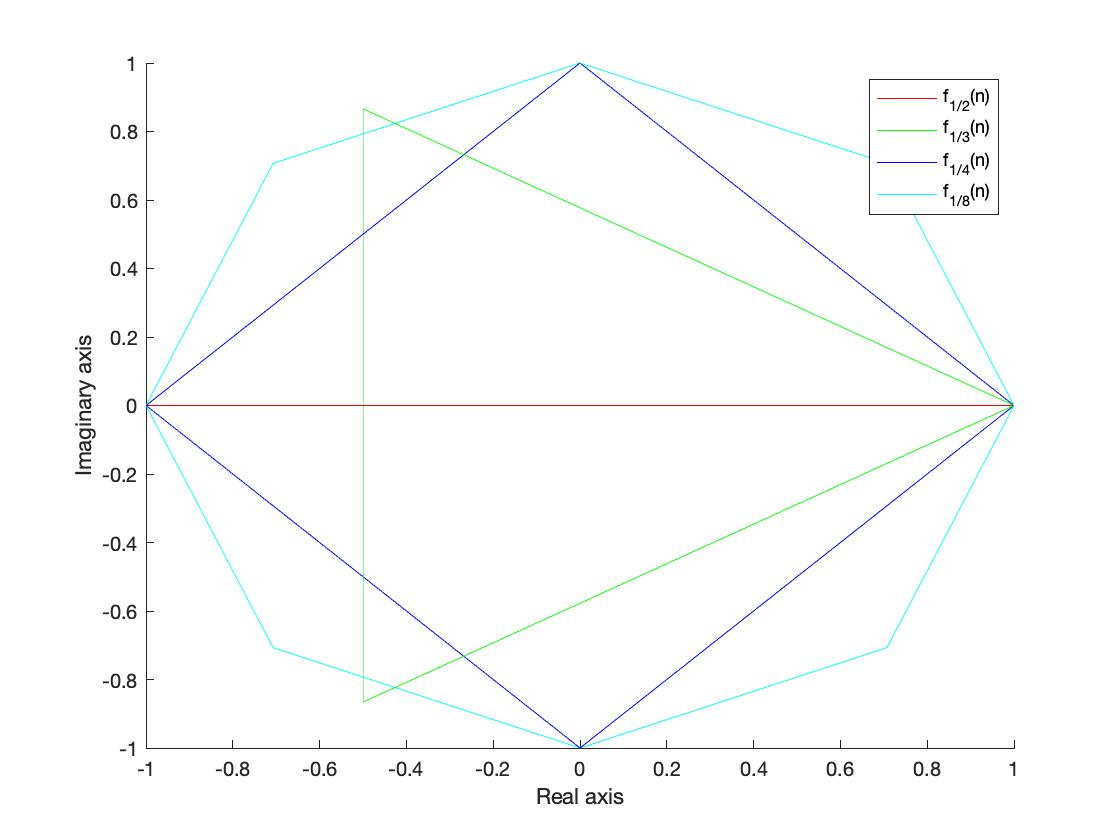
\includegraphics[width = 0.75\linewidth]{plot_2D}
	\caption{2D plot of $f_\omega(n)$. It is possible to seen that each function is evaluated at the corresponding roots of unity. }
	\label{fig:plot1}
	\end{figure}
	
	\begin{figure}[h!]
	\centering
	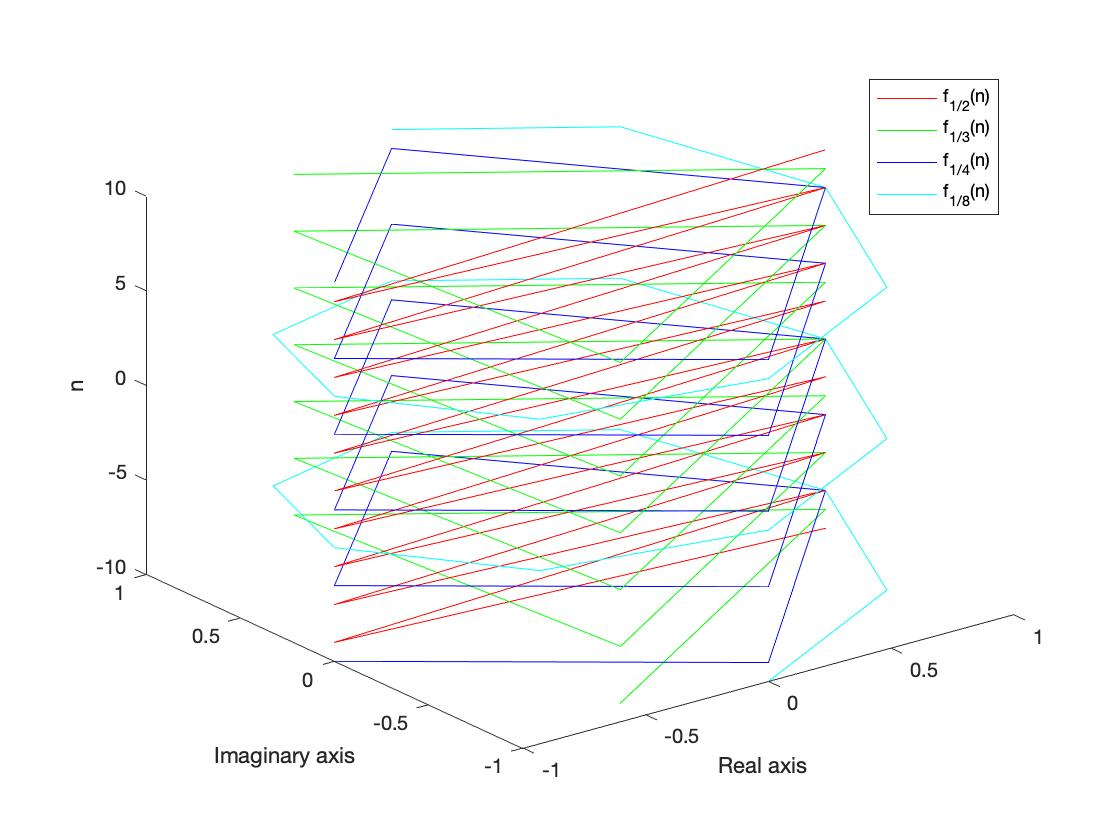
\includegraphics[width = 0.75\linewidth]{plot_3D}
	\caption{3D plot of $f_\omega(n)$.}
	\label{fig:plot2}
	\end{figure}
	\newpage
	\textbf{b} A function $f(x)$ is said to be periodic if for a constant $D \in \mathbb{R}$ it follows that 
	
	$$f(x) = f(x+D), \qquad \forall x \in f$$
	
	Then, for the concrete case of this exercise, $f_\omega (n)$ is periodic if:
	
	$$ f_\omega (n) = f_\omega (n + N), \qquad  \forall n \in \mathbb{Z}$$
	
	$$\implies e^{2\pi i \omega n} = e^{2\pi i \omega (n+N)}$$
	
	$$ e^{2\pi i \omega n} = e^{2\pi i \omega n} e^{2\pi i \omega N} $$
	
	The latter implies that:
	
	$$e^{2\pi i \omega N} = 1, \qquad \forall N \in \mathbb{Z}$$
	
	Additionally, since $e^{2\pi i x} = 1, \qquad \forall x \in \mathbb{Z}$:
	
	$$2\pi i \omega N = 2\pi i x$$
	
	$$N\omega = x$$
	
	$$ \omega = \frac{x}{N} $$
	
	Since $x$ and $N \in \mathbb{Z}$, then $\omega$ has to be in $\mathbb{Q}$ so the function is periodic. \hfill $\qed$

	\section*{Exercise 3.3}
	\textbf{a.} Knowing that $\cos(x) = \frac{1}{2}\left(e^{ix} + e^{-ix}\right)$ and that $(a+b)^3 = a^3 + 3a^2b + 3ab^2 + b^3$, then:
	
	\begin{alignat*}{2}
	\cos^3(x) &= \left(\frac{1}{2}\right)^3 (e^{ix} + e^{-ix})^3\\
	&= \frac{1}{8} \left(e^{3ix}+3e^{2ix}e^{-ix} + 3e^{ix}e^{-2ix}+e^{-3ix}\right)\\
	&= \frac{1}{8} \left(e^{3ix}+e^{-3ix} + 3e^{ix} + 3e^{-ix}\right)\\
	&= \frac{1}{8} \left(e^{3ix}+e^{-3ix}\right) + \frac{3}{8}\left(e^{ix} + e^{-ix}\right)\\
	&= \frac{1}{4} \cdot \frac{1}{2} \left(e^{3ix}+e^{-ix3}\right) +  \frac{3}{4} \cdot \frac{1}{2}\left(e^{ix} + e^{-ix}\right)\\
	&= \frac{1}{4} \cos(3x) +  \frac{3}{4}  \cos(x) & 
	\end{alignat*} \hfill $ \qed$
	

\end{document}
